\begin{activity} \label{A:9.7.9} A {\em central force} is one that
  acts on an object so that the force $\vF$ is parallel to the
  object's position $\vr$.  Since Newton's Second Law says that an
  object's acceleration is proportional to the force exerted on it,
  the acceleration $\va$ of an object moving under a central force
  will be parallel to its position $\vr$.  For instance, the Earth's
  acceleration due to the 
  gravitational force that the sun exerts on the Earth is parallel to
  the Earth's position vector as shown in Figure \ref{F:9.7.sun}.

\begin{figure}[ht]
  \begin{center}
    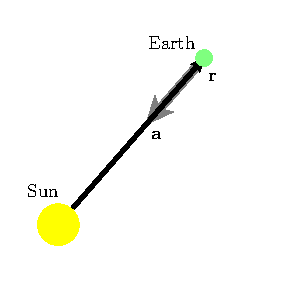
\includegraphics{figures/fig_9_7_sun.eps}
    \caption{A central force.}
    \label{F:9.7.sun}
  \end{center}
\end{figure}

\ba
\item If an object of mass $m$ is moving under a central force, 
  the angular momentum vector is defined to be $\vL=m\vr\times\vv$.
  Assuming the mass is constant, show that the angular momentum is
  constant by showing that
  $$
  \frac{d\vL}{dt} = 0.
  $$

\item Explain why $\vL\cdot\vr = 0$.

\item Explain why we may conclude that the object is constrained to
  lie in the plane passing through the origin and perpendicular to
  $\vL$.





\ea

\end{activity}
\begin{smallhint}

\end{smallhint}
\begin{bighint}

\end{bighint}
\begin{activitySolution}
   \ba
    \item The quantity $\vr(t+h)-\vr(t)$ is a vector quantity, the vector from the terminal point of $\vr(t)$ to the terminal point of $\vr(t+h)$.

    \item The quantity $\frac{\vr(t+h)-\vr(t)}{h}$ is a vector quantity, it is a vector in the direction of $\vr(t+h)-\vr(t)$ that is $\frac{1}{h}$ times as long. 

    \item The vector $\vr(t+h)-\vr(t)$ represents a change in position of the object on the time interval $[t, t+h]$. When we multiply by $\frac{1}{h}$, we can consider this vector  $\frac{\vr(t+h)-\vr(t)}{h}$ as an average change of position, or the average velocity vector of the object on the interval $[t,t+h]$. 

    \item As $h \to 0$, the average velocity vectors $\frac{\vr(t+h)-\vr(t)}{h}$ approach the instantaneous velocity vector. The average velocity vector $\frac{\vr(t+h)-\vr(t)}{h}$ is a direction vector for the secant line to the curve that passes through the terminal points of $\vr(t)$ and $\vr(t+h)$. As we let $h \to 0$, these direction vectors approach a direction vector  
        \[\ds \lim_{h \to 0} \frac{\vr(t+h)-\vr(t)}{h}\]
of the tangent line to the curve at the terminal point of $\vr(t)$. 
    \ea

\end{activitySolution}
\aftera
